\documentclass[
	a4paper,
	oneside,
	BCOR = 10mm,
	DIV = 12,
	12pt,
	headings = normal,
]{scrartcl}

%%% Length calculations
\usepackage{calc}
%%%

%%% Support for color
\usepackage{xcolor}
\definecolor{lightblue}{HTML}{03A9F4}
\definecolor{red}{HTML}{F44336}
%%%

%%% Including graphics
\usepackage{graphicx}
%%%

%%% Font selection
\usepackage{fontspec}

\setromanfont{STIX Two Text}[
	SmallCapsFeatures = {LetterSpace = 8},
]

\setsansfont{IBM Plex Sans}[
	Scale = MatchUppercase,
]

\setmonofont{IBM Plex Mono}[
	Scale = MatchUppercase,
]
%%%

%%% Math typesetting
\usepackage{amsmath}

\usepackage{unicode-math}
\setmathfont{STIX Two Math}
%%%

%%% List settings
\usepackage{enumitem}
\setlist[enumerate]{
	label*      = {\arabic*.},
	leftmargin  = *,
	labelindent = \parindent,
	topsep      = 1\baselineskip,
	parsep      = 0\baselineskip,
	itemsep     = 1\baselineskip,
}

\setlist[itemize]{
	label*      = {—},
	leftmargin  = *,
	labelindent = \parindent,
	topsep      = 1\baselineskip,
	parsep      = 0\baselineskip,
	itemsep     = 1\baselineskip,
}

\setlist[description]{
	font        = {\rmfamily\upshape\bfseries},
	topsep      = 1\baselineskip,
	parsep      = 0\baselineskip,
	itemsep     = 0\baselineskip,
}

%%%

%%% Structural elements typesetting
\setkomafont{pagenumber}{\rmfamily}
\setkomafont{disposition}{\rmfamily\bfseries}

% Sectioning
\RedeclareSectionCommand[
	beforeskip = -1\baselineskip,
	afterskip  = 1\baselineskip,
	font       = {\normalsize\bfseries\scshape},
]{section}

\RedeclareSectionCommand[
	beforeskip = -1\baselineskip,
	afterskip  = 1\baselineskip,
	font       = {\normalsize\bfseries\itshape},
]{subsection}

\RedeclareSectionCommand[
	beforeskip = -1\baselineskip,
	afterskip  = 1\baselineskip,
	font       = {\normalsize\bfseries},
]{subsubsection}

\RedeclareSectionCommand[
	beforeskip = -1\baselineskip,
	afterskip  = -0.5em,
	font       = {\normalsize\mdseries\scshape\addfontfeatures{Letters = {UppercaseSmallCaps}}},
]{paragraph}
%%%

%%% Typographic enhancements
\usepackage{microtype}
%%%

%%% Language-specific settings
\usepackage{polyglossia}
\setmainlanguage{ukrainian}
\setotherlanguages{english}
%%%

%%% Captions
\usepackage{caption}
\usepackage{subcaption}

%\DeclareCaptionLabelFormat{closing}{#2)}
%\captionsetup[subtable]{labelformat = closing}

%\captionsetup[subfigure]{labelformat = closing}

\captionsetup[table]{
	aboveskip = 0\baselineskip,
	belowskip = 0\baselineskip,
}

\captionsetup[figure]{
	aboveskip = 1\baselineskip,
	belowskip = 0\baselineskip,
}

\captionsetup[subfigure]{
	labelformat = simple,
	labelformat = brace,
}
%%%

%%% Table typesetting
\usepackage{booktabs}
\usepackage{longtable}

\usepackage{multirow}

\usepackage{array}
\newcolumntype{v}[1]{>{\raggedright\arraybackslash\hspace{0pt}}p{#1}}
\newcolumntype{b}[1]{>{\centering\arraybackslash\hspace{0pt}}p{#1}}
\newcolumntype{n}[1]{>{\raggedleft\arraybackslash\hspace{0pt}}p{#1}}
%%%

%%% Drawing with TikZ
\usepackage{tikz}
\usepackage{tikzscale}
\usetikzlibrary{
	arrows.meta, % Stealth arrow tips
	positioning,
	shapes,
	trees,
}

\tikzset{> = stealth}

\tikzset{
	actor/.style = {
		rounded rectangle,
		draw,
		% fill = white,
		font = \small,
		minimum height = 4\baselineskip,
		minimum width = 3\gridunitwidth,
		text width = 3\gridunitwidth,
		align = center,
	}
}

\tikzset{
	service/.style = {
		rectangle,
		draw,
		% fill = white,
		font = \small,
		minimum height = 4\baselineskip,
		minimum width = 3\gridunitwidth,
		text width = 3\gridunitwidth,
		align = center,
	}
}

\tikzset{
	hiernode/.style = {
		rectangle,
		draw,
		% fill = white,
		font = \small,
		minimum height = 3\baselineskip,
		minimum width = 2\gridunitwidth,
		text width = 2\gridunitwidth,
		align = center,
	}
}
%%%

%%% Drawing forests (hierarchiel diagram
\usepackage{forest}

%%%

%%% PDF inclusion
\usepackage{pdfpages}
%%%

%%% Links and hyperreferences
\usepackage{hyperref}
\hypersetup{
	bookmarksnumbered = true,
	colorlinks      = false,
	linkbordercolor = red,
	urlbordercolor  = lightblue,
	pdfborderstyle  = {/S/U/W 1.5},
}
%%%

%%% Length adjustments
% Set baselineskip, default is 14.5 pt
\linespread{1.068966} % ~15.5 pt
\setlength{\emergencystretch}{1em}
\setlength{\parindent}{1.5em}
\newlength{\gridunitwidth}
\setlength{\gridunitwidth}{\textwidth / 12}
%%%

%%% Custom commands
\newcommand{\allcaps}[1]{{\addfontfeatures{LetterSpace = 8, Kerning = Off}#1}}
%%%

\begin{document}
	\begin{titlepage}
		\begin{center}
			Міністерство освіти і науки України\\
			Національний авіаційний університет\\
			Навчально-науковий інститут комп'ютерних інформаційних технологій\\
			Кафедра комп'ютеризованих систем управління

			\vspace{\fill}
				Лабораторна робота №1.2\\
				з дисципліни «Інженерія програмного забезпечення»\\
				на тему «Розробка вимог до програмної системи»\\
				Варіант №3

			\vspace{\fill}

			\begin{flushright}
				Виконав:\\
				студент ННІКІТ\\
				групи СП-325\\
				Клокун В.\,Д.\\
				Перевірила:\\
				Голего Н.\,М.
			\end{flushright}

			Київ 2018
		\end{center}
	\end{titlepage}

	\section{Мета}
		Вивчити підходи до~складання проекту вимог до~інформаційної системи, оформити технічне завдання на~розробку програмного забезпечення.

	\section{Завдання}
		Скласти проект вимог до~інформаційної системи, оформити технічне завдання на~розробку програмного забезпечення, оформити звіт з~лабораторної роботи.
		
	\section{Хід роботи}
		Визначаємо опорні точки зору на~основі методу \textenglish{Viewpoint Oriented Requirements Defintion~(\allcaps{VORD})}. За~визначеними опорними точками зору, будуємо діаграми ідентифікації точок зору~(рис.~\ref{fig:diagram-viewpoint-id}) та~ієрархії точок зору~(рис.~\ref{fig:diagram-viewpoint-hierarchy}).
		
		На основі опису системи~(результат виконання лабораторної роботи~№1.1), створених діаграм та~вимог складаємо технічне завдання на~розробку інформаційної системи аеропорту.

		\begin{figure}[!htbp]
			\centering
			\begin{tikzpicture}
				\node [actor] (passenger) {Пасажир};
				\node [service, left = 1\gridunitwidth of passenger.west] (flight-status-data-view) {Перегляд даних про статус рейсу};

				\node [actor, below = 1\baselineskip of passenger] (operator-atc) {Оператор модуля~«Повітряний рух»};
				\node [service, left = 1\gridunitwidth of operator-atc] (air-pos-data) {Отримання даних про місцезнаходження повітряного судна};
				\node [service, right = 1\gridunitwidth of operator-atc] (air-pos-data) {Редагування даних повітряного руху};

				\node [actor, below = 1\baselineskip of operator-atc] (operator-log) {Оператор модуля~«Логістика»};
				\node [service, left = 1\gridunitwidth of operator-log] (flight-status-data-in-airport-view) {Перегляд даних про повітряне судно в аеропорті};
				\node [service, right = 1\gridunitwidth of operator-log] (flight-status-data-in-airport-view) {Редагування логістичних даних};

				\node [actor, below = 1\baselineskip of operator-log] (operator-ctl) {Оператор модуля~«Керування»};
				\node [service, left = 1\gridunitwidth of operator-ctl] (flight-status-data-in-airport-view) {Перегляд статусу підключених модулів};
				
				% \node [service, below = 1\baselineskip of air-pos-data] (flight-status-data) {Отримання даних про статус рейсу};
				% \node [service, below = 1\baselineskip of flight-status-data] (aircraft-inflight-data-view) {Перегляд даних про повітряне судно в польоті};
			\end{tikzpicture}
			\caption{Діаграма ідентифікації точок зору}
			\label{fig:diagram-viewpoint-id}
		\end{figure}

		\begin{figure}[!htbp]
			\centering
			\begin{tikzpicture}
				\node [hiernode] (root) {Усі точки зору};
				\node [hiernode, left = 1\gridunitwidth of root, yshift = -4\baselineskip] (client) {Клієнт};
				\node [hiernode, below = 1\baselineskip of client] (passenger) {Пасажир};

				\node [hiernode, right = 1\gridunitwidth of root, yshift = -4\baselineskip] (workers) {Працівники};
				\node [hiernode, below = 1\baselineskip of workers] (operator-log) {Оператор модуля «Логістика»};
				\node [hiernode, left = 1\gridunitwidth of operator-log] (operator-ctl) {Оператор модуля «Керування»};
				\node [hiernode, right = 1\gridunitwidth of operator-log] (operator-atc) {Оператор модуля «Повітряний рух»};

				\draw[->] (root) -- (client);
				\draw[->] (root) -- (workers);

				\draw[->] (client) -- (passenger);

				\draw[->] (workers) -- (operator-ctl);
				\draw[->] (workers) -- (operator-log);
				\draw[->] (workers) -- (operator-atc);
			\end{tikzpicture}
			\caption{Діаграма ієрархії точок зору}
			\label{fig:diagram-viewpoint-hierarchy}
		\end{figure}

	\section{Висновок}
		Під час виконання даної лабораторної роботи ми вивчили підходи до~складання проекту вимог до~інформаційної системи, оформили технічне завдання на~розробку програмного забезпечення.

	\newpage

	\appendix
	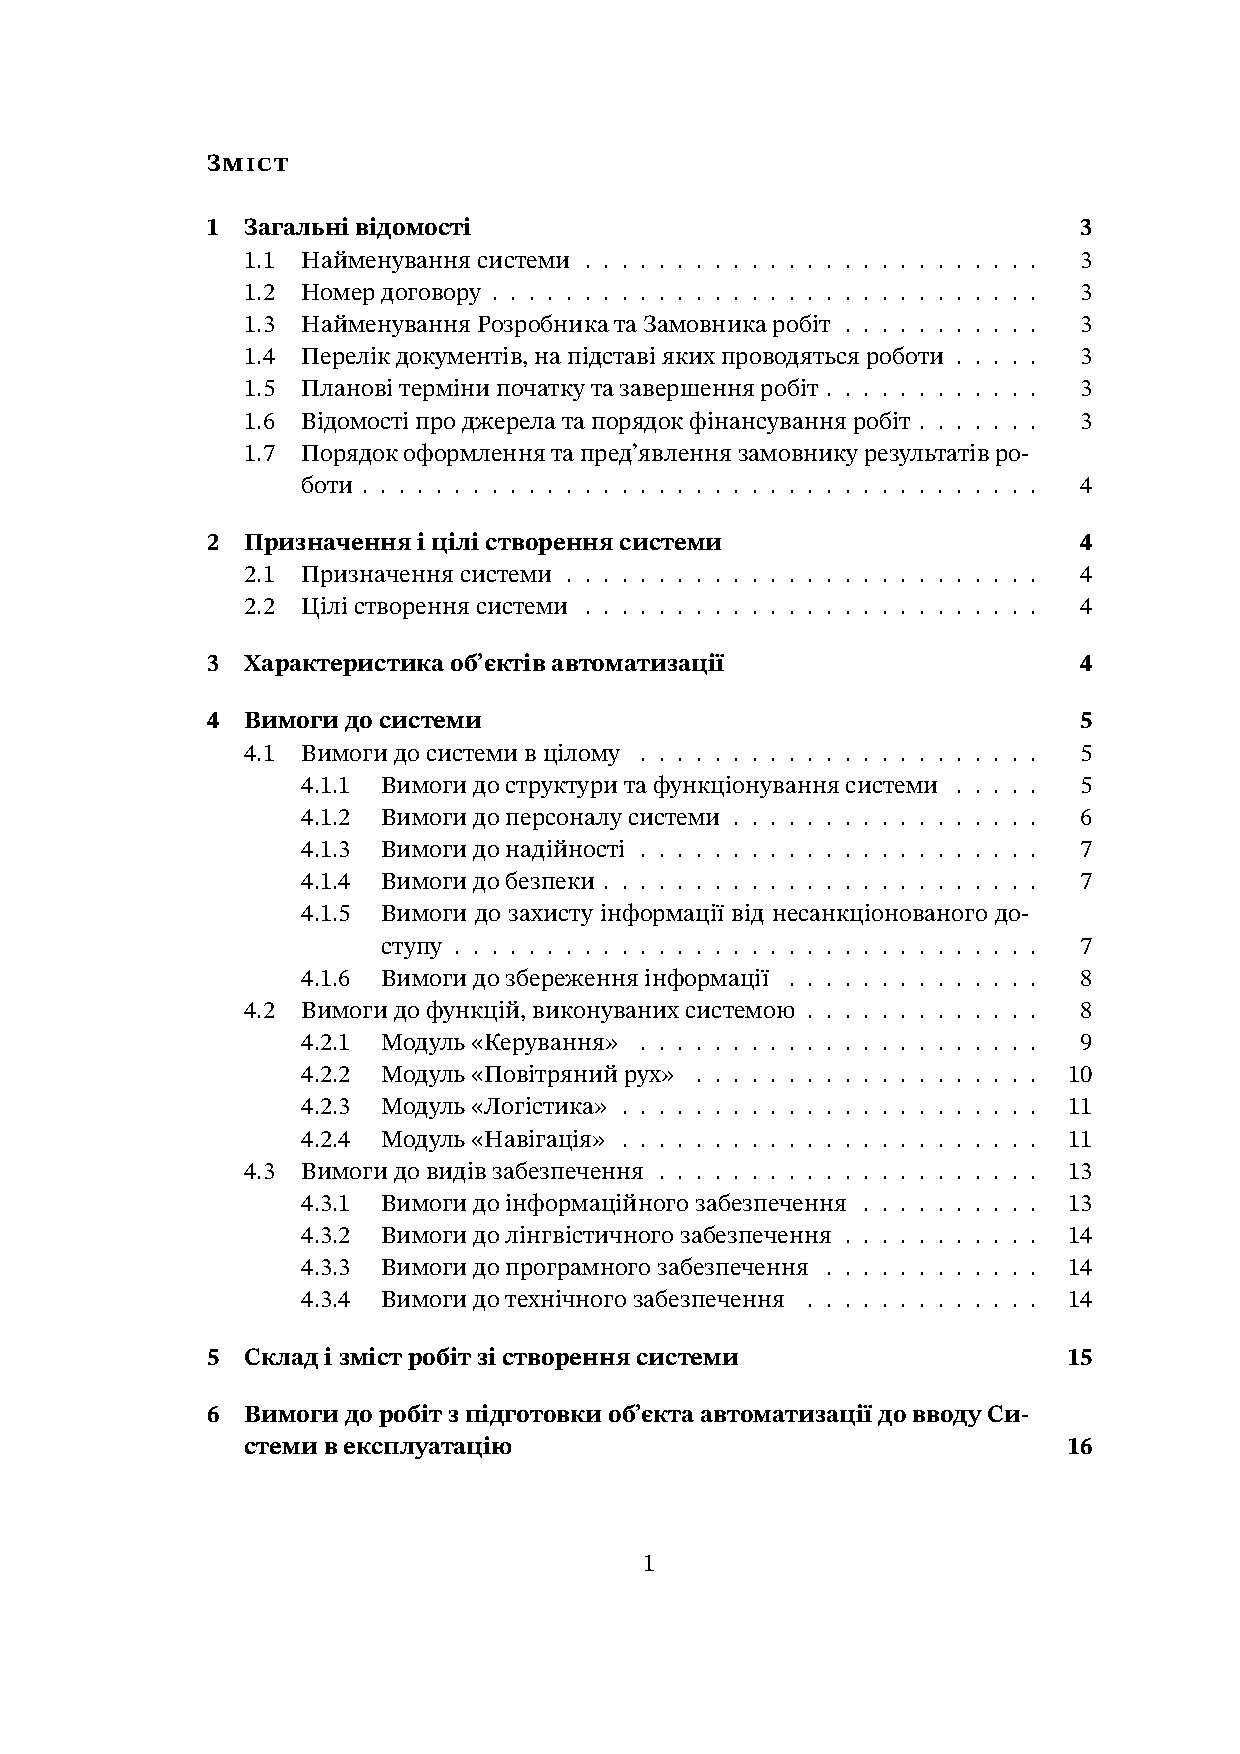
\includepdf[pages=-]{y03s01-softeng-lab-02-report-add-01-prd.pdf}

\end{document}
